% This LaTeX was auto-generated from MATLAB code.
% To make changes, update the MATLAB code and export to LaTeX again.

\documentclass{article}

\usepackage[utf8]{inputenc}
\usepackage[T1]{fontenc}
\usepackage{lmodern}
\usepackage{graphicx}
\usepackage{color}
\usepackage{hyperref}
\usepackage{amsmath}
\usepackage{amsfonts}
\usepackage{epstopdf}
\usepackage[table]{xcolor}
\usepackage{matlab}

\sloppy
\epstopdfsetup{outdir=./}
\graphicspath{ {./HW11_code_images/} }

\matlabhastoc

\matlabmultipletitles

\begin{document}
	
\maketitle
\thispagestyle{empty}
\pagebreak
\matlabtableofcontents{Table of Contents}

\begin{par}
\begin{flushleft}
In this homework assignment a Kohonen Self-Organizing Map (SOM) will be trained on MNIST dataset and the resulting weights of the network (centroids) will be dispalyed as images.
\end{flushleft}
\end{par}

\begin{matlabcode}
clc; clear; close all;
load('HW11_code_workspace.mat');
\end{matlabcode}
\pagebreak


\label{T_AF22880B}
\matlabtitle{0. MNIST Dataset}

\label{H_FBA02D0E}
\matlabheading{0.1 Downloading MNIST Dataset and Importing into \textit{Matlab}}

\begin{par}
\begin{flushleft}
The code snippet below will download MNIST dataset from web and extract the downloaded files into Matlab matrices as test and train images and labels.
\end{flushleft}
\end{par}

\begin{matlabcode}
mnist_train_image = 'train-images-idx3-ubyte';
mnist_train_label = 'train-labels-idx1-ubyte';
mnist_test_image  = 't10k-images-idx3-ubyte';
mnist_test_label  = 't10k-labels-idx1-ubyte';
train_set_number  = 60000;
test_set_number   = 10000;

downloadMNIST(mnist_train_image, mnist_train_label, mnist_test_image, mnist_test_label);
\end{matlabcode}
\begin{matlaboutput}
MNIST dataset already downloaded.
\end{matlaboutput}


\begin{matlabcode}
[train_images, train_labels] = readMNIST(mnist_train_image, mnist_train_label, train_set_number);

clear mnist_train_image mnist_train_label mnist_test_image mnist_test_label train_set_number test_set_number
\end{matlabcode}


\label{H_3C76610B}
\matlabheading{0.2 Plotting a Sample of MNIST Dataset}

\begin{par}
\begin{flushleft}
A set of 100 randomly chosen samples of the training dataset is plotted here.
\end{flushleft}
\end{par}

\begin{matlabcode}
random_indices = randi(60000, [1 100]);
montage(train_images(:, :, random_indices), 'BorderSize', [2 2], 'BackgroundColor', 'white');
\end{matlabcode}
\begin{center}
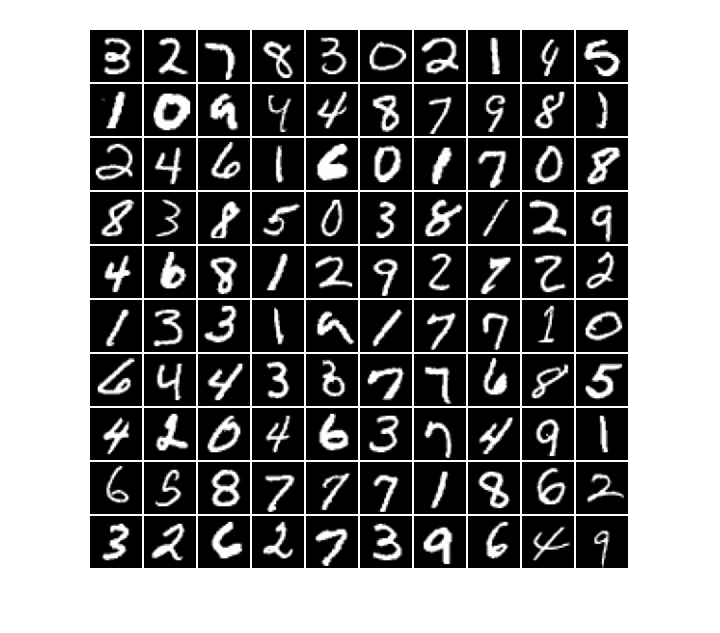
\includegraphics[scale=0.5]{figure_0.png}
\end{center}


\label{H_FC5FEF34}
\matlabheading{0.3 Number of Occurances for Each Digit in Training Set}

\begin{par}
\begin{flushleft}
Here we investigate how many of each digit is there in the training set.
\end{flushleft}
\end{par}

\begin{matlabcode}
for i=0:9
    disp([num2str(i),': ', num2str(sum(train_labels == i))]);
end
\end{matlabcode}
\begin{matlaboutput}
0: 5923
1: 6742
2: 5958
3: 6131
4: 5842
5: 5421
6: 5918
7: 6265
8: 5851
9: 5949
\end{matlaboutput}
\pagebreak

\label{T_D3238000}
\matlabtitle{1,2. Training Kohonen SOM}

\label{H_2E8C4985}
\matlabheading{1,2.1 Reshaping the Training images}

\begin{par}
\begin{flushleft}
The images should be reshaped from 28x28 images to vectors of 784 elements, so they could be fed into our neural network.
\end{flushleft}
\end{par}

\begin{matlabcode}
train_images_reshaped = reshape(train_images, [size(train_images, 1)*size(train_images, 2) size(train_images, 3)]);
\end{matlabcode}


\label{H_4C731258}
\matlabheading{1,2.2 Defining the Network}

\begin{par}
\begin{flushleft}
The Self-Organizing Map (SOM) charactersitics are defined as below:
\end{flushleft}
\end{par}

\begin{itemize}
\setlength{\itemsep}{-1ex}
   \item{\begin{flushleft} SOM's number of output neurons is 40. \end{flushleft}}
   \item{\begin{flushleft} The network will be trained for 2000 epochs on the whole training set of MNIST and the neighborhood size will be shrinked to 1 on the 1000th epoch and maintained 1 for the rest of training process. \end{flushleft}}
   \item{\begin{flushleft} Initial number of neighbors for each neuron (window size) is set to 31. \end{flushleft}}
   \item{\begin{flushleft} The SOM output is distributed on a line (1-D). \end{flushleft}}
\end{itemize}

\begin{matlabcode}
net = selforgmap(40, 1000, 31, 'gridtop', 'dist');
net.trainParam.showCommandLine = true;
net = configure(net, train_images_reshaped);
\end{matlabcode}


\begin{par}
\begin{flushleft}
The SOM block diagram is shown below.
\end{flushleft}
\end{par}

\begin{matlabcode}
view(net);
\end{matlabcode}

\begin{par}
\begin{flushleft}
\centering
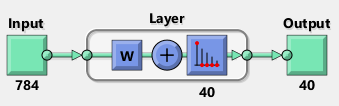
\includegraphics[scale=0.7]{image_0}
\end{flushleft}
\end{par}
\pagebreak

\label{H_D6F54383}
\matlabheading{1,2.3 Training the Network}

\begin{par}
\begin{flushleft}
Training process is started here and will perform 2000 epochs on the whole training set of MNIST.
\end{flushleft}
\end{par}

\begin{matlabcode}
[net, tr] = train(net, train_images_reshaped, 'showResources', 'yes');
\end{matlabcode}
\begin{matlaboutput}
Calculation mode: MATLAB
 
Training Self-Organizing Map with TRAINBU.
Epoch 0/2000, Time 8.554
Epoch 25/2000, Time 197.912
Epoch 50/2000, Time 388.029
Epoch 75/2000, Time 578.313
Epoch 100/2000, Time 768.036
Epoch 125/2000, Time 957.678
Epoch 150/2000, Time 1147.487
Epoch 175/2000, Time 1328.154
Epoch 200/2000, Time 1503.661
Epoch 225/2000, Time 1679.494
Epoch 250/2000, Time 1870.152
Epoch 275/2000, Time 2059.483
Epoch 300/2000, Time 2249.092
Epoch 325/2000, Time 2438.753
Epoch 350/2000, Time 2626.825
Epoch 375/2000, Time 2813.981
Epoch 400/2000, Time 3002.164
Epoch 425/2000, Time 3178.537
Epoch 450/2000, Time 3351.311
Epoch 475/2000, Time 3527.981
Epoch 500/2000, Time 3715.781
Epoch 525/2000, Time 3907.704
Epoch 550/2000, Time 4100.043
Epoch 575/2000, Time 4284.706
Epoch 600/2000, Time 4467.254
Epoch 625/2000, Time 4658.501
Epoch 650/2000, Time 4851.395
Epoch 675/2000, Time 5043.137
Epoch 700/2000, Time 5234.683
Epoch 725/2000, Time 5428.209
Epoch 750/2000, Time 5621.437
Epoch 775/2000, Time 5814.927
Epoch 800/2000, Time 6007.923
Epoch 825/2000, Time 6212.168
Epoch 850/2000, Time 6406.661
Epoch 875/2000, Time 6603.632
Epoch 900/2000, Time 6800.42
Epoch 925/2000, Time 7047.682
Epoch 950/2000, Time 7295.847
Epoch 975/2000, Time 7527.051
Epoch 1000/2000, Time 7761.811
Epoch 1025/2000, Time 8004.686
Epoch 1050/2000, Time 8241.381
Epoch 1075/2000, Time 8462.575
Epoch 1100/2000, Time 8664.065
Epoch 1125/2000, Time 8861.952
Epoch 1150/2000, Time 9050.906
Epoch 1175/2000, Time 9240.2
Epoch 1200/2000, Time 9430.527
Epoch 1225/2000, Time 9620.054
Epoch 1250/2000, Time 9809.33
Epoch 1275/2000, Time 10004.54
Epoch 1300/2000, Time 10194.7
Epoch 1325/2000, Time 10383.463
Epoch 1350/2000, Time 10573.368
Epoch 1375/2000, Time 10762.671
Epoch 1400/2000, Time 10952.85
Epoch 1425/2000, Time 11139.882
Epoch 1450/2000, Time 11326.853
Epoch 1475/2000, Time 11515.307
Epoch 1500/2000, Time 11699.105
Epoch 1525/2000, Time 11882.011
Epoch 1550/2000, Time 12065.211
Epoch 1575/2000, Time 12247.955
Epoch 1600/2000, Time 12431.069
Epoch 1625/2000, Time 12614.593
Epoch 1650/2000, Time 12798.048
Epoch 1675/2000, Time 12972.773
Epoch 1700/2000, Time 13145.682
Epoch 1725/2000, Time 13318.952
Epoch 1750/2000, Time 13492.329
Epoch 1775/2000, Time 13665.607
Epoch 1800/2000, Time 13839.321
Epoch 1825/2000, Time 14012.678
Epoch 1850/2000, Time 14186.349
Epoch 1875/2000, Time 14366.093
Epoch 1900/2000, Time 14550.599
Epoch 1925/2000, Time 14741.273
Epoch 1950/2000, Time 14925.515
Epoch 1975/2000, Time 15109.601
Epoch 2000/2000, Time 15292.645
Training with TRAINBU completed: Maximum epoch reached.
 
\end{matlaboutput}
\pagebreak

\label{T_D9DAA2AE}
\matlabtitle{3. Displaying 40 Centroids}

\label{H_40BD747F}
\matlabheading{3.1 Saving Weights for Further Use}

\begin{par}
\begin{flushleft}
Every neuron in the output layer will have a set of weights of 784 elements. We will save and reshape them in images of 28x28 size.
\end{flushleft}
\end{par}

\begin{matlabcode}
weights = net.IW{1}';
weights_reshaped = reshape(weights, [28 28 40]);
\end{matlabcode}
\pagebreak

\label{H_E4179F93}
\matlabheading{3.2 Plotting Weights (Centroids)}

\begin{par}
\begin{flushleft}
The whole training dataset is mapped into 40 neurons. Here we have plotted the centroids. A number above every centroid represents the number of images of the training dataset which are mapped into that specific centroid.
\end{flushleft}
\end{par}

\begin{matlabcode}
y = net(train_images_reshaped);
map_results = sum(y, 2);

figure('Position', [1, 1, 1000, 1000]);
for i = 1:40
    subplot(6, 7, i);
    imshow(weights_reshaped(:, :, i));
    t = sprintf('%d: %d', i, map_results(i));
    title(t);
    hold on;
end
hold off
\end{matlabcode}
\begin{center}
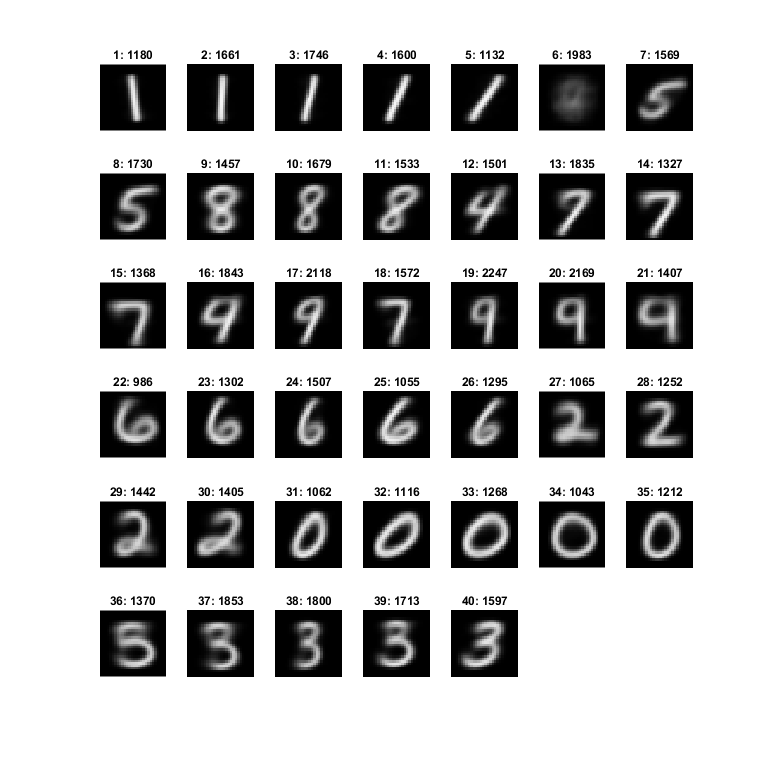
\includegraphics[scale=0.5]{figure_1.png}
\end{center}
\pagebreak

\label{T_F8AA430C}
\matlabtitle{Appendix}

\label{H_64B544B3}
\matlabheading{A.1 Saving Workspace Variables for Future Use }

\begin{matlabcode}
save('HW11_code_workspace.mat')
\end{matlabcode}


\label{H_430FCF21}
\matlabheading{A.2 Defiition of Auxiliary Functions}

\begin{matlabcode}
function downloadMNIST(mnist_train_image, mnist_train_label, mnist_test_image, mnist_test_label)

if exist('train-images-idx3-ubyte','file') ~= 2
    disp('Downloading MNIST dataset...');
    websave([mnist_train_image,'.gz'],...
        ['http://yann.lecun.com/exdb/mnist/', ...
        mnist_train_image, '.gz']);
    websave([mnist_train_label,'.gz'],...
        ['http://yann.lecun.com/exdb/mnist/', ...
        mnist_train_label, '.gz']);
    websave([mnist_test_image,'.gz'],...    
        ['http://yann.lecun.com/exdb/mnist/', ...
        mnist_test_image, '.gz']);
    websave([mnist_test_label,'.gz'],...
        ['http://yann.lecun.com/exdb/mnist/', ...
        mnist_test_label, '.gz']);
    disp('MNIST dataset downloded.');
    
    disp('Unzipping started...');
    gunzip([mnist_train_image, '.gz'])
    gunzip([mnist_train_label, '.gz'])
    gunzip([mnist_test_image, '.gz'])
    gunzip([mnist_test_label, '.gz'])
    delete([mnist_train_image, '.gz'])
    delete([mnist_train_label, '.gz'])
    delete([mnist_test_image, '.gz'])
    delete([mnist_test_label, '.gz'])
    disp('Unzipping completed.');
else
    disp('MNIST dataset already downloaded.')
end

end

function [imgs, labels] = readMNIST(imgFile, labelFile, num_of_digits_to_read)

fileID = fopen(imgFile, 'r', 'b');
header = fread(fileID, 1, 'int32');

if header ~= 2051
    error('Invalid image file header');
end

count = fread(fileID, 1, 'int32');

if count < num_of_digits_to_read
    error('Trying to read too many digits');
end

rows_num = fread(fileID, 1, 'int32');
cols_num = fread(fileID, 1, 'int32');

imgs = zeros([rows_num cols_num num_of_digits_to_read]);

for i = 1:num_of_digits_to_read
    for row = 1:rows_num
        imgs(row, :, i) = fread(fileID, cols_num, 'uint8');
    end
end

fclose(fileID);

fileID = fopen(labelFile, 'r', 'b');
header = fread(fileID, 1, 'int32');

if header ~= 2049
    error('Invalid label file header');
end

count = fread(fileID, 1, 'int32');

if count < num_of_digits_to_read
    error('Trying to read too many digits');
end

labels = fread(fileID, num_of_digits_to_read, 'uint8');

fclose(fileID);

imgs = double(imgs)./255.0;

end

function iMontage(images)
montage(reshape(images, [28 28 size(images, 2)]), 'BackgroundColor', 'white', 'BorderSize', [2 2]);
end

function display_original_images_vs_reconstructed(original_images, reconstructed_images)
figure('Position', [100, 100, 1000, 500]);
subplot(1, 2, 1);
iMontage(original_images);
title('Original Images');
hold on;
subplot(1, 2, 2);
iMontage(reconstructed_images);
title('Reconstructed Images')
hold off
end

function categorized_label = iCategorical(on_hot_encoded_label)
[ind, ~]= vec2ind(on_hot_encoded_label);
categorized_label = categorical(ind', 1:10, {'0' '1' '2' '3' '4' '5' '6' '7' '8' '9'});
end




function saveMNISTasFolderOfImages(outputPath, train_images, train_labels, test_images, test_labels)

if(~isempty(outputPath))
    assert(exist(outputPath,'dir') == 7);
end

% Set names for directories
trainDirectoryName = 'mnistTrain';
testDirectoryName = 'mnistTest';

% Create directories for the output
mkdir(fullfile(outputPath, trainDirectoryName));
mkdir(fullfile(outputPath, testDirectoryName));

labelNames = {'0','1','2','3','4','5','6','7','8','9'};
iMakeTheseDirectories(fullfile(outputPath, trainDirectoryName), labelNames);
iMakeTheseDirectories(fullfile(outputPath, testDirectoryName), labelNames);


iLoadBatchAndWriteAsImagesToLabelFolders(train_images, fullfile(outputPath, trainDirectoryName), labelNames, train_labels);

iLoadBatchAndWriteAsImagesToLabelFolders(test_images, fullfile(outputPath, testDirectoryName), labelNames, test_labels);

end

function iLoadBatchAndWriteAsImagesToLabelFolders(data, fullOutputDirectoryPath, labelNames, labels)
for i = 1:size(data,3)
    imwrite(data(:,:,i), fullfile(fullOutputDirectoryPath, labelNames{labels(i)+1}, ['image' num2str(i) '.png']));
end
end

function iMakeTheseDirectories(outputPath, directoryNames)
for i = 1:numel(directoryNames)
    mkdir(fullfile(outputPath, directoryNames{i}));
end
end

\end{matlabcode}

\end{document}
